% !TEX root = ReviewDraft.tex



\section{Entropy of radiation}


 
We have seen how the black hole   fine-grained entropy,  as computed via the gravitational formula \eqref{RT},  accurately follows the Page curve. This does not directly address the information paradox since that concerns the entropy growth of the Hawking radiation. 
In fact, the semi-classical black hole evolution leads to a growing value for the entropy outside the cutoff surface, the region containing the radiation \cite{Hawking:1976ra}, 
\be 
 \Ssemi(\Sigma_{\rm Rad})\,. \la{SemiRad}
 \ee 
This radiation lives in a spacetime region where the gravitational effects can be made very small. In other words, we can approximate this as a rigid space. Alternatively, we can think we collected the radiation into a big quantum computer.  
   However,   due to the fact that we used   gravity to obtain this state, it turns out that we should apply the gravitational  fine-grained entropy formula to compute its entropy.  
   In our first presentation of the formula \nref{RT}, we were imagining that we had a black hole inside the region. Now we are trying to apply this formula to the region outside the cutoff surface, which contains no black hole. Nevertheless, the formula \nref{RT} can also be applied when there is no black hole present.  The spirit of the formula is that the region in which we compute the entropy can be changed in size, by moving the surface $X$, so as to minimize the entropy. So far we have considered cases where $\Sigma_X$ was connected. However, it seems also natural to consider the possibility that $\Sigma_X$ is disconnected. When would this be required? By making $\Sigma_X$ disconnected, we increase the area of the boundary. So this can only be required if we can decrease the semiclassical entropy contribution at the same time. This could happen if we have regions that are far away with entangled matter. 
   In fact, this is precisely what happens with Hawking radiation. The radiation is entangled with the fields living in the black hole interior. Therefore, we can decrease the semiclassical entropy contribution by also including the black hole interior. In doing so, we will have to add an area term.   At late times, the net effect is to decrease the generalized entropy, so we are required to include this disconnected region inside the black hole, which is sometimes called an ``island." The final region we are considering looks as in figure \ref{islandprocedure}. 
   
   More precisely,  the full  fine-grained entropy of the radiation, computed using the  fine-grained gravitational entropy formula, is given by 
\begin{align}
S_\mathrm{Rad} = \mathrm{min}_X \Bigg\{ \mathrm{ext}_X\left[ {\mathrm{Area}(X) \over 4 \GN} + \Ssemi [\Sigma_{\rm Rad} \,  \cup \,  \Sigma_{\rm Island}] \right] \Bigg\}, \label{island}
\end{align}
where the area here refers to the area of the boundary of the island, and the min/ext is with respect to the location and shape of the island \cite{Almheiri:2019hni,Penington:2019kki,Almheiri:2019qdq} . 
The left hand side is the full entropy of radiation.  
 And $\Ssemi [\Sigma_{\rm Rad} \,  \cup \,  \Sigma_{\rm Island}]    $ is the von Neumann entropy of the quantum state of the combined radiation and island systems {\it in the semiclassical description}. 
Note that the subscript `Rad' appears both on the left hand side and the right hand side of \nref{island}, a fact that has caused much confusion and heated complaints. The left hand side is the full entropy of radiation, as computed using the gravitational  fine-grained entropy formula. This is supposed to be the entropy for the full exact quantum state of the radiation.  On the right hand side we have the state of radiation {\it in the semiclassical description}. This is a different state than the full exact state of the radiation. Note that in order to apply the formula we do not need to know the exact state of the radiation. The formula does not claim to give that state  to us in an explicit form, it is only computing the entropy of that state.  
  


\begin{figure}[t]
\begin{center}
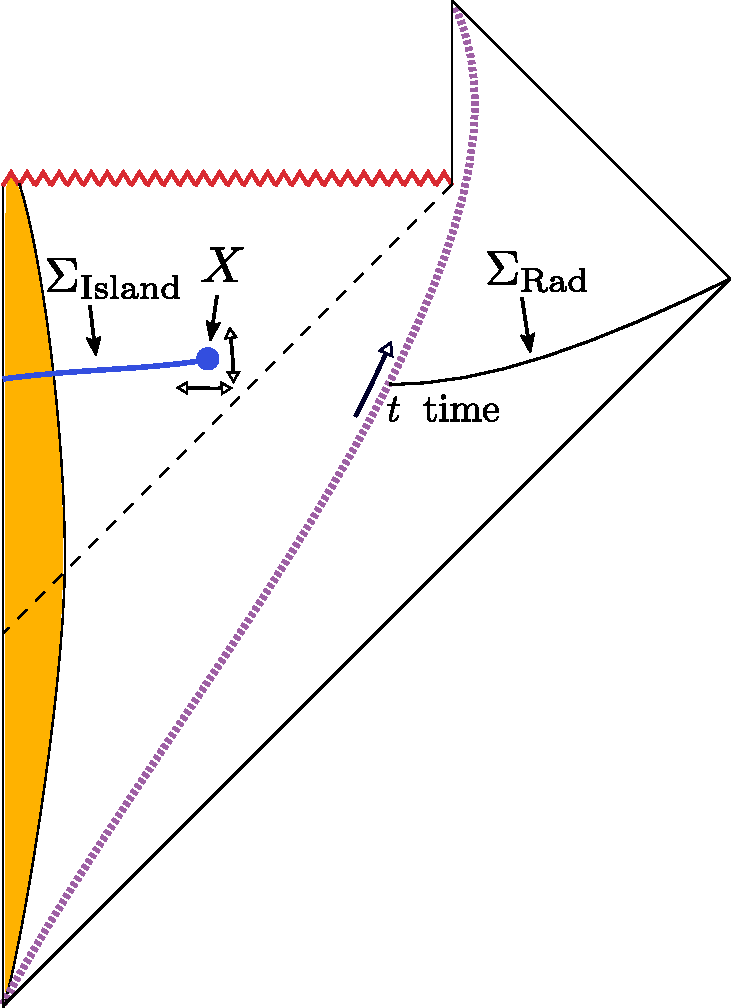
\includegraphics[scale=0.4]{figures/islandprocedure.pdf}
\caption{The  fine-grained entropy of the region Rad containing the Hawking radiation can get contributions from regions inside the black hole, called islands. The total entropy is the area of $X$ plus a   contribution from the semiclassical entropy of the union of $\Sigma_{\rm Rad}$ and $\Sigma_{\rm Island}$.}
\label{islandprocedure}
\end{center}
\end{figure}

The ``island formula'' \nref{island} is a generalization of the black hole gravitational  fine-grained entropy formula \nref{RT} and really follows from the same principles. Some authors consider it as simply a part of \nref{RT}. We decided to give it a special name and to discuss it separately because we motivated \nref{RT} as a generalization of black hole entropy. However, if we look just at the radiation, there does not seem to be any black hole.  The point is that because we prepared the state using gravity, this is the correct formula to use. We will later give a sketch of the derivation of the formula. It is likely that in future treatments of the subject, both will be discussed together. 

 
The procedure for applying this formula is as follows. We want to compute the entropy of all of the Hawking radiation that has escaped the black hole region. This is captured by computing the entropy of the entire region from the cutoff all the way to infinity. This region is labeled by $\Sigma_{\rm Rad}$  in the formula, see figure \ref{islandprocedure}. The islands refer to any number of regions contained in the black hole side of the cutoff surface. The figure shows the case of a single island centered around the origin. In principle we can have any number of islands, including zero. We then extremize the right hand side of 
\nref{island} with respect to the position of the surface $X$. Finally we minimize over all possible extremal positions and choices of islands. 

The simplest possibility is to have no island. 
This vanishing island contribution gives simply \nref{SemiRad}.   As more and more outgoing Hawking quanta escape the black hole region, the entropy continues to grow. See figure \ref{radnoisland}. This contribution always extremizes the generalized entropy but it will not always be the global minimum of the entropy. 

\begin{figure}[t]
\begin{center}
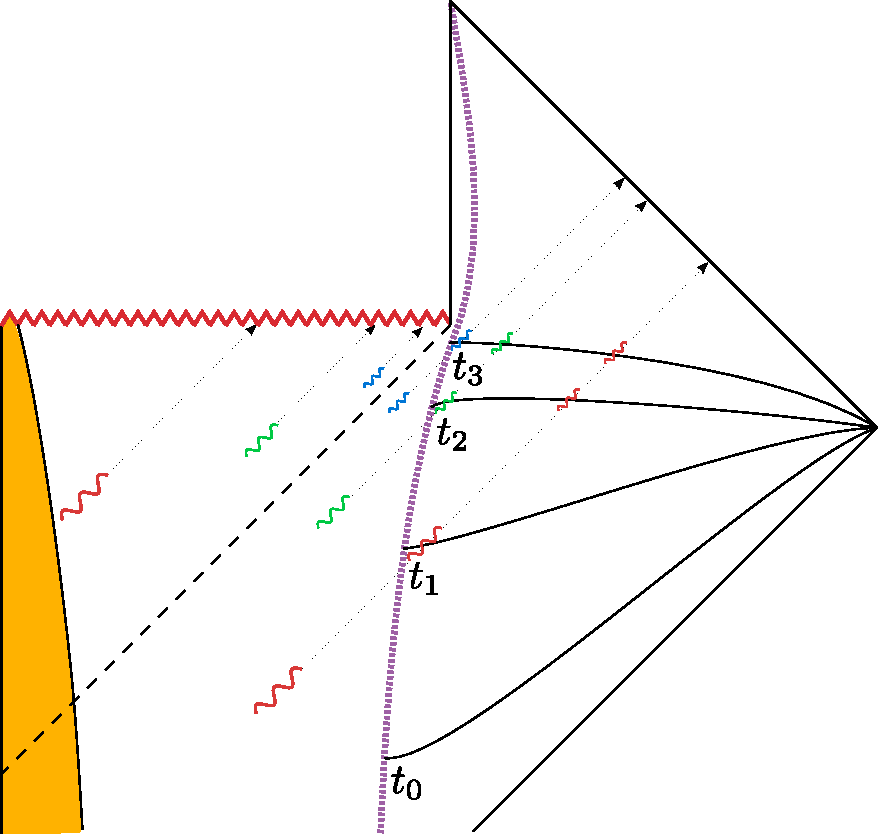
\includegraphics[scale=0.4]{figures/radnoisland.pdf}
 \ \ \ \ \ \  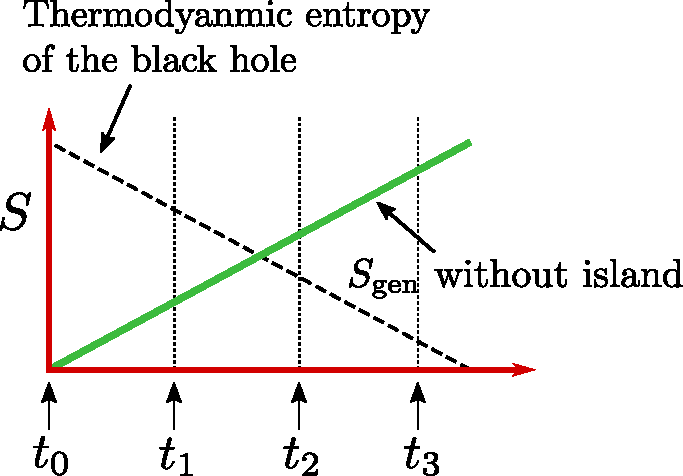
\includegraphics[scale=0.6]{figures/radnoislandcurve.pdf}
\caption{The no-island contribution to the island formula gives a growing entropy due to the escaping outgoing Hawking quanta.  }
\label{radnoisland}
\end{center}
\end{figure}



A non-vanishing island that extremizes the generalized entropy appears some time after the black hole forms. A time of order $r_s \log S_{BH}$ is enough. This island is centered around the origin and its boundary is very near the black hole event horizon. It moves up the horizon for different times on the cutoff surface. This is shown in figure \ref{radwithisland}. The generalized entropy with this island includes the term which is given by the area of the black hole. The von Neumann entropy term involves the entropy of the union of the outgoing radiation and the island, and is therefore small for all times, since the island contains most or all of the interior Hawking modes that purify the outgoing radiation. This contribution to the island formula starts at a large value, given by the area of the horizon at early times, and decreases down to zero.

\begin{figure}[htbp]
\begin{center}
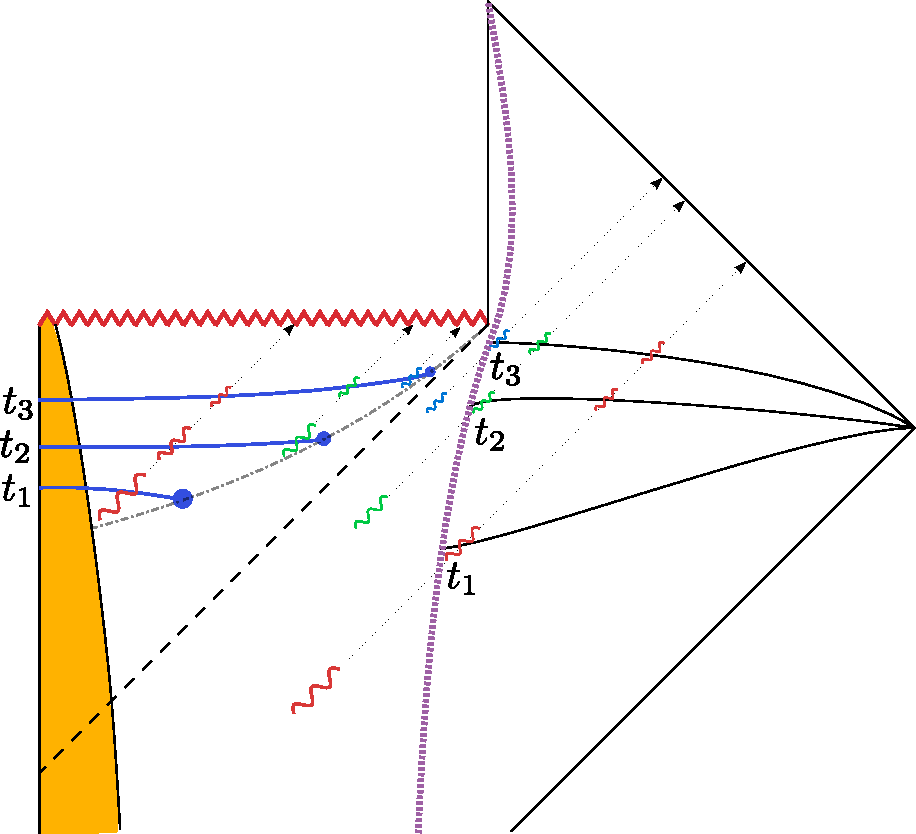
\includegraphics[scale=0.4]{figures/radwithisland.pdf}
 \ \ \ \ \ \  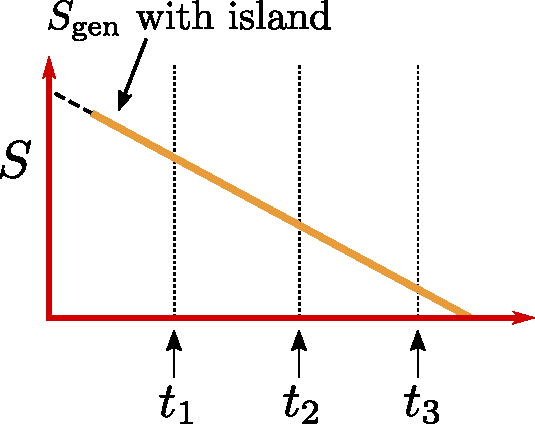
\includegraphics[scale=0.6]{figures/radwithislandcurve.pdf}
\caption{The  island contribution appears some time after the black hole forms. It gives a decreasing contribution that tracks the thermodynamic entropy of the black hole.   }
\label{radwithisland}
\end{center}
\end{figure}

\begin{figure}[htbp]
\begin{center}
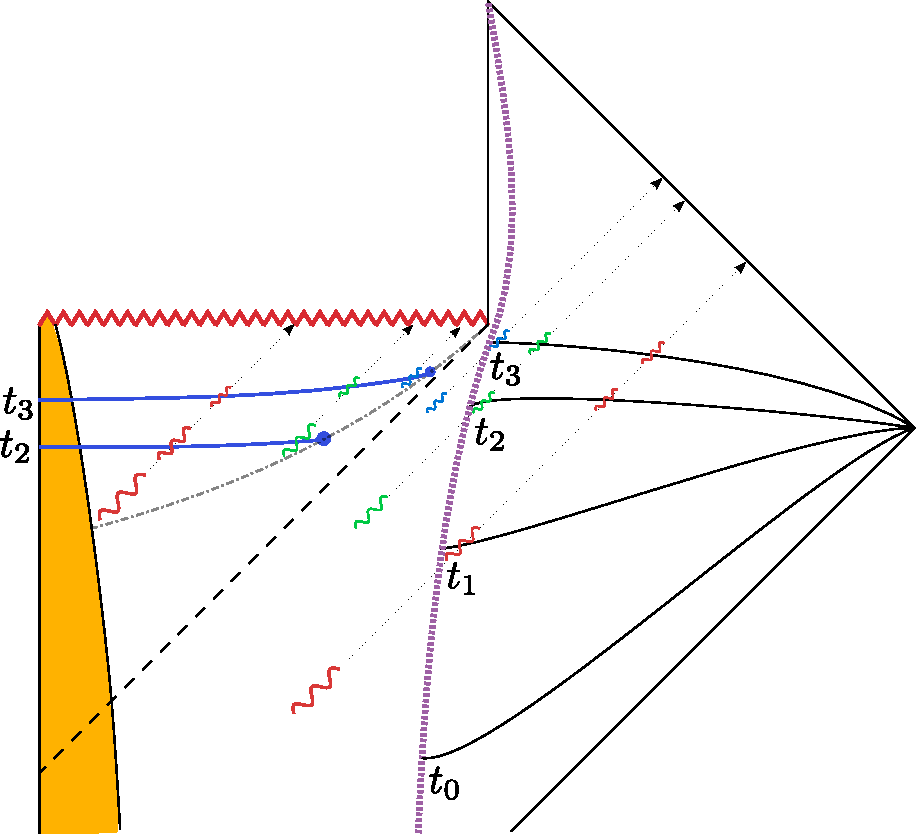
\includegraphics[scale=0.4]{figures/islandtransition.pdf}
 \ \ \ \ \ \ 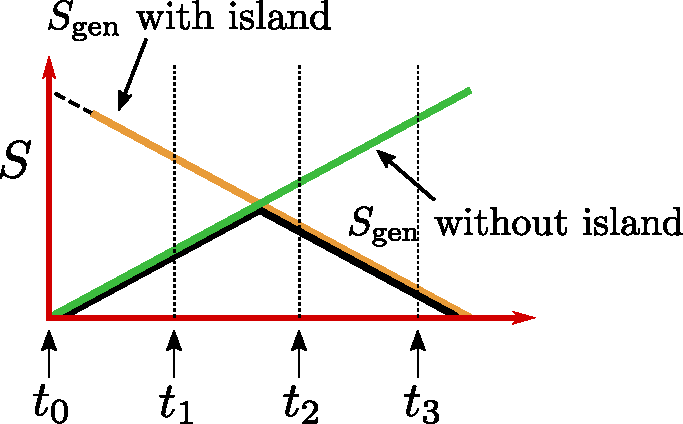
\includegraphics[scale=0.6]{figures/islandtransitioncurve.pdf}
\caption{ We now consider both contributions and at each time we pick the minimal one, which gives the final answer for the full entropy of radiation.   This gives the Page curve, shown in black on the right figure.    }
\label{radboth}
\end{center}
\end{figure}


The  fine-grained entropy of the Hawking radiation is then   the minimum of these two contributions. This gives the Page curve; the rising piece comes from  the no-island contribution and the novel decreasing piece from the island contribution. 

 
If we formed the black hole from an initially pure state, then we expect that the entropy of the black hole and the entropy of the radiation  region should be equal. 
 Indeed, the fine grained entropy formula for the black hole and the one for the radiation give the same answer. The reason is the following. In both cases,  the same surface $X$ is involved. In addition, When the matter state is pure on the whole Cauchy slice,  we have that 
  $\Ssemi(\Sigma_X) = \Ssemi(\Sigma_\textup{Rad} \cup \Sigma_\textup{Island})$. Then we get the same answer because we are minimizing/extremizing the same function. 
 In conclusion, the black hole and the radiation entropy are described by the same curve, see figure \ref{HawkingPageCurves}. 


 

Now a skeptic would say: ``Ah, all you have done is to include the interior region. As I have always been saying, if you include the interior region you get a pure state,"  or ``This is only an accounting trick." But we did not include the interior ``by hand." The  fine-grained entropy formula is derived from the gravitational path integral through a method conceptually similar to the derivation of the black hole entropy by Gibbons and Hawking, discussed in section \ref{ss:gibbonshawking}. It is gravity itself, therefore, that instructs us to include the interior in this calculation. 
It is gravity's way of telling us that black hole evaporation is unitary without giving us the details of the actual state of the outgoing radiation.





An analogy from the real world is the following. Imagine that there is a man who owns a house with many expensive paintings inside. Then he starts borrowing money from the townspeople giving the paintings as a guarantee. He spends his money throwing expensive parties and people who visit his house think he is very rich. However, he eventually borrows so much that most of the house and its contents belong to the townspeople. So, when the townspeople  compute their wealth, they include the paintings in this man's house. But the man cannot include them in his computation of his wealth. 
In this analogy, the house is the interior of the black hole and the wealth is the quantum information. The townspeople is the region far from the black hole containing the Hawking radiation.  The casual observer who thinks that the townspeople are poor because they don't have paintings in their homes would be wrong.  In the same way,  the one who looks at the Hawking radiation and said that it is mixed would be wrong, because the interior should also be included. 
 

 
  

